\documentclass[a4paper, 12pt]{article}

\usepackage[left=2cm,right=2cm,
    top=2cm,bottom=2cm,bindingoffset=0cm]{geometry}

\usepackage[T2A]{fontenc}
\usepackage[utf8]{inputenc}
\usepackage{color}
\usepackage{graphicx}
\usepackage{caption}
\usepackage{subcaption}
\usepackage{tikz}
\usepackage[english, russian]{babel}
\usepackage{ gensymb }
\usepackage{booktabs}
\usepackage{amsmath,amsfonts,amssymb,amsthm,mathtools}
\usepackage{lscape}

\begin{document}
% ТИТУЛЬНИК %
	\pagestyle{empty}
	\begin{center}
		МИНИСТЕРСТВО ОБРАЗОВАНИЯ И НАУКИ РОССИЙСКОЙ ФЕДЕРАЦИИ \\ ГОСУДАРСТВЕННОЕ БЮДЖЕТНОЕ ОБРАЗОВАТЕЛЬНОЕ УЧРЕЖДЕНИЕ \\ 
		ВЫСШЕГО ПРОФЕССИОНАЛЬНОГО ОБРАЗОВАНИЯ
		\vskip 1.5cm
		«Московский государственный технический \\
		университет имени Н.Э. Баумана» \\
		(МГТУ им. Н.Э. Баумана)
		\vskip 1.5cm
		ФАКУЛЬТЕТ ФУНДАМЕНТАЛЬНЫЕ НАУКИ \\
		КАФЕДРА \\
		«ВЫЧИСЛИТЕЛЬНАЯ МАТЕМАТИКА И МАТЕМАТИЧЕСКАЯ ФИЗИКА»
		\vskip 0.4cm
		Направление: \textbf{Математика и компьютерные науки}
		\vskip 0.4cm
		Дисциплина: Основы метода конечных элементов
		\vskip 0.4cm
		Лабораторная работа 1 \\
		«Дискретные одномерные элементы» \\
		Группа ФН11-71Б
		\vskip 0.2cm
		Вариант 7
		
		
		\vskip 1.5cm
		\begin{flushright}
			Студент: Долотова А.А.
			
			\vskip 1.5cm
			
			Преподаватель: Захарова Ю.В.
		\end{flushright}
		Оценка:
		
		\begin{figure}[b]
			\begin{center}
				Москва, 2024
			\end{center}
		\end{figure}
		
	\end{center}
	
	% ТИТУЛЬНИК %
	\newpage
	\pagestyle{plain}

\begin{center}
\textbf{\textit{Задание}}
\end{center}

Дана исследуемая область с граничными условиям ($T_{\text{среды}}$ или $T_{\text{ср}}$ равносильно теплообмену со средой). Геометрические параметры области $A, B, L, a, b$ [см] задаются самостоятельно. Воздействие теплового потока принять равным  $q = 150$ [Вт/$\text{см}^2$], коэффициент теплоотдачи от стенки к среде 
$\alpha_g = 10 [\text{Вт/(см)}^2\cdot$ \celsius]; $T$ – заданная температура стенки, 150 [\celsius] ;  $T_{\text{среды}} = 25$ [\celsius] -- температура окружающей среды,  $\lambda = 75 [\text{Вт/(см)}\cdot$ \celsius]  - коэффициент теплопроводности материала. \\

Требуется:
\begin{enumerate}
\item	Провести дискретизацию области дискретными одномерными элементами.
\itemВыписать уравнения равновесия для нескольких элементов.
\itemЗаписать несколько локальных матриц: для внутренних элементов, граничных элементов и локальных векторов правых частей.
\itemОписать процедуру формирования глобальной матрицы теплопроводности и правых частей.
\itemПолучить СЛАУ для решения методом Гаусса и Холецкого.
\itemНайти распределение температуры в исследуемой области, решив полученное СЛАУ. 
\end{enumerate}

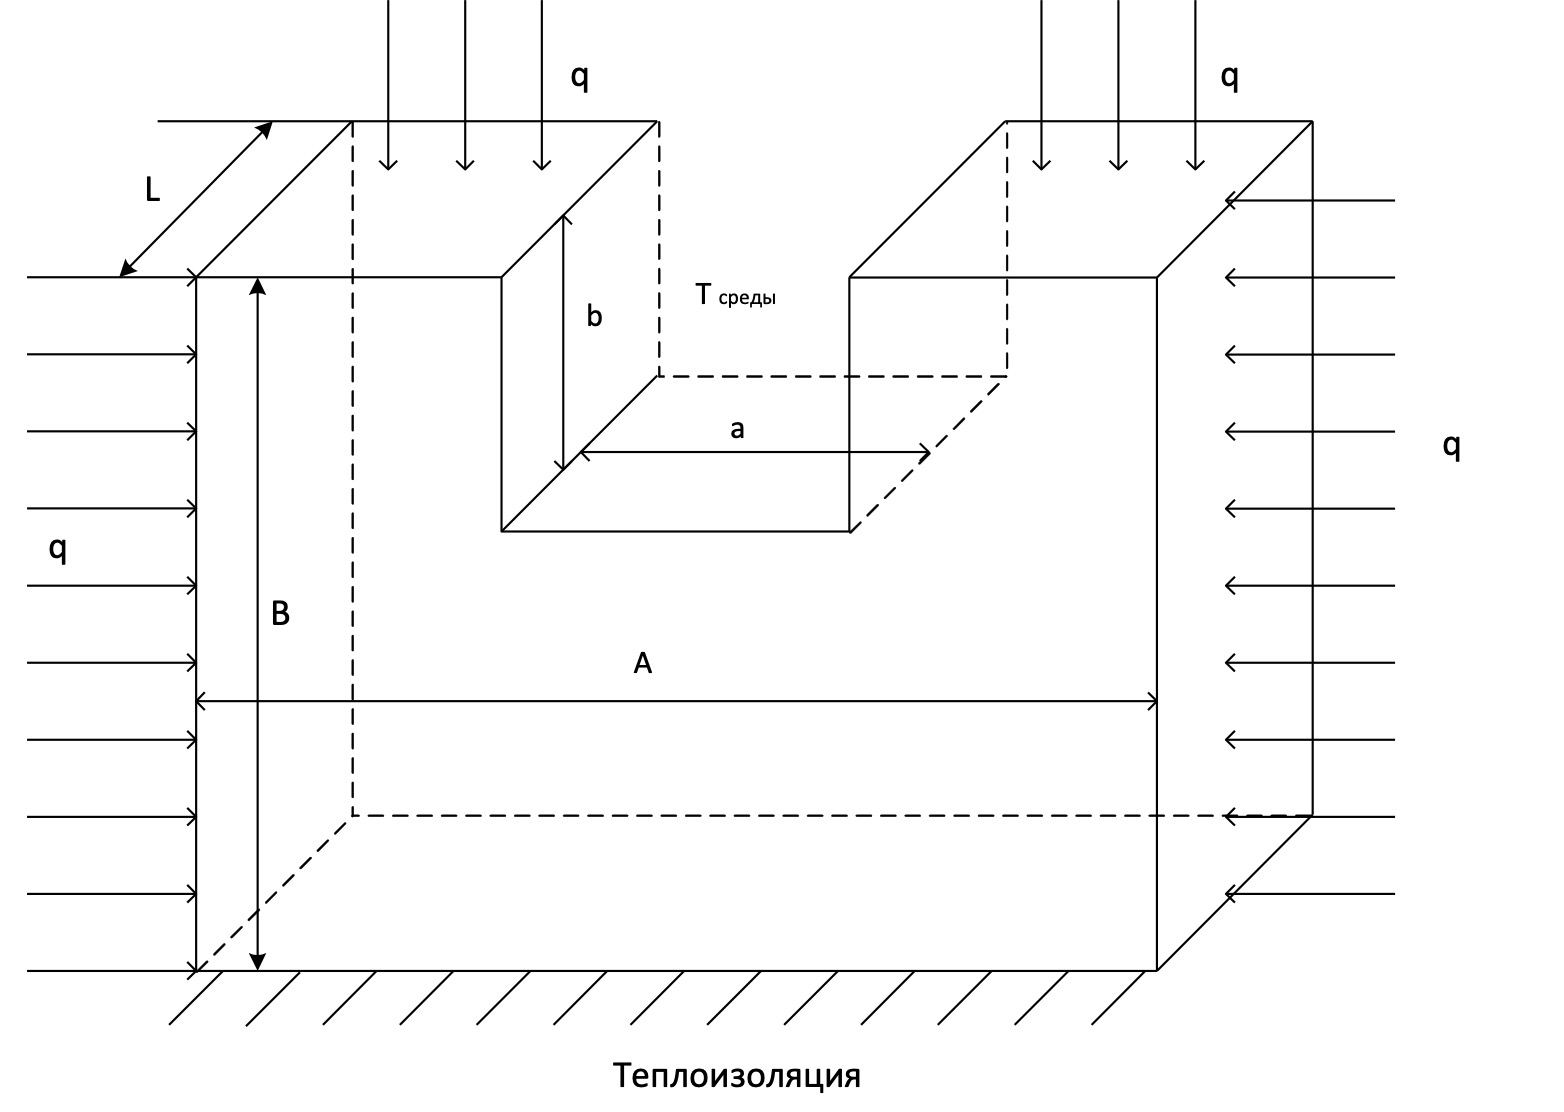
\includegraphics[width=1\textwidth]{img1.jpeg}

\newpage

\begin{center}
\textbf{\textit{Решение}}
\end{center}

Пусть $L=1, A=6, B=4, a=2, b=2$.

Разделим исходную область на две симметричные части и будем рассматривать одну из них. Грань
поверхности разреза будем считать абсолютно теплоизолированной.

\begin{center}
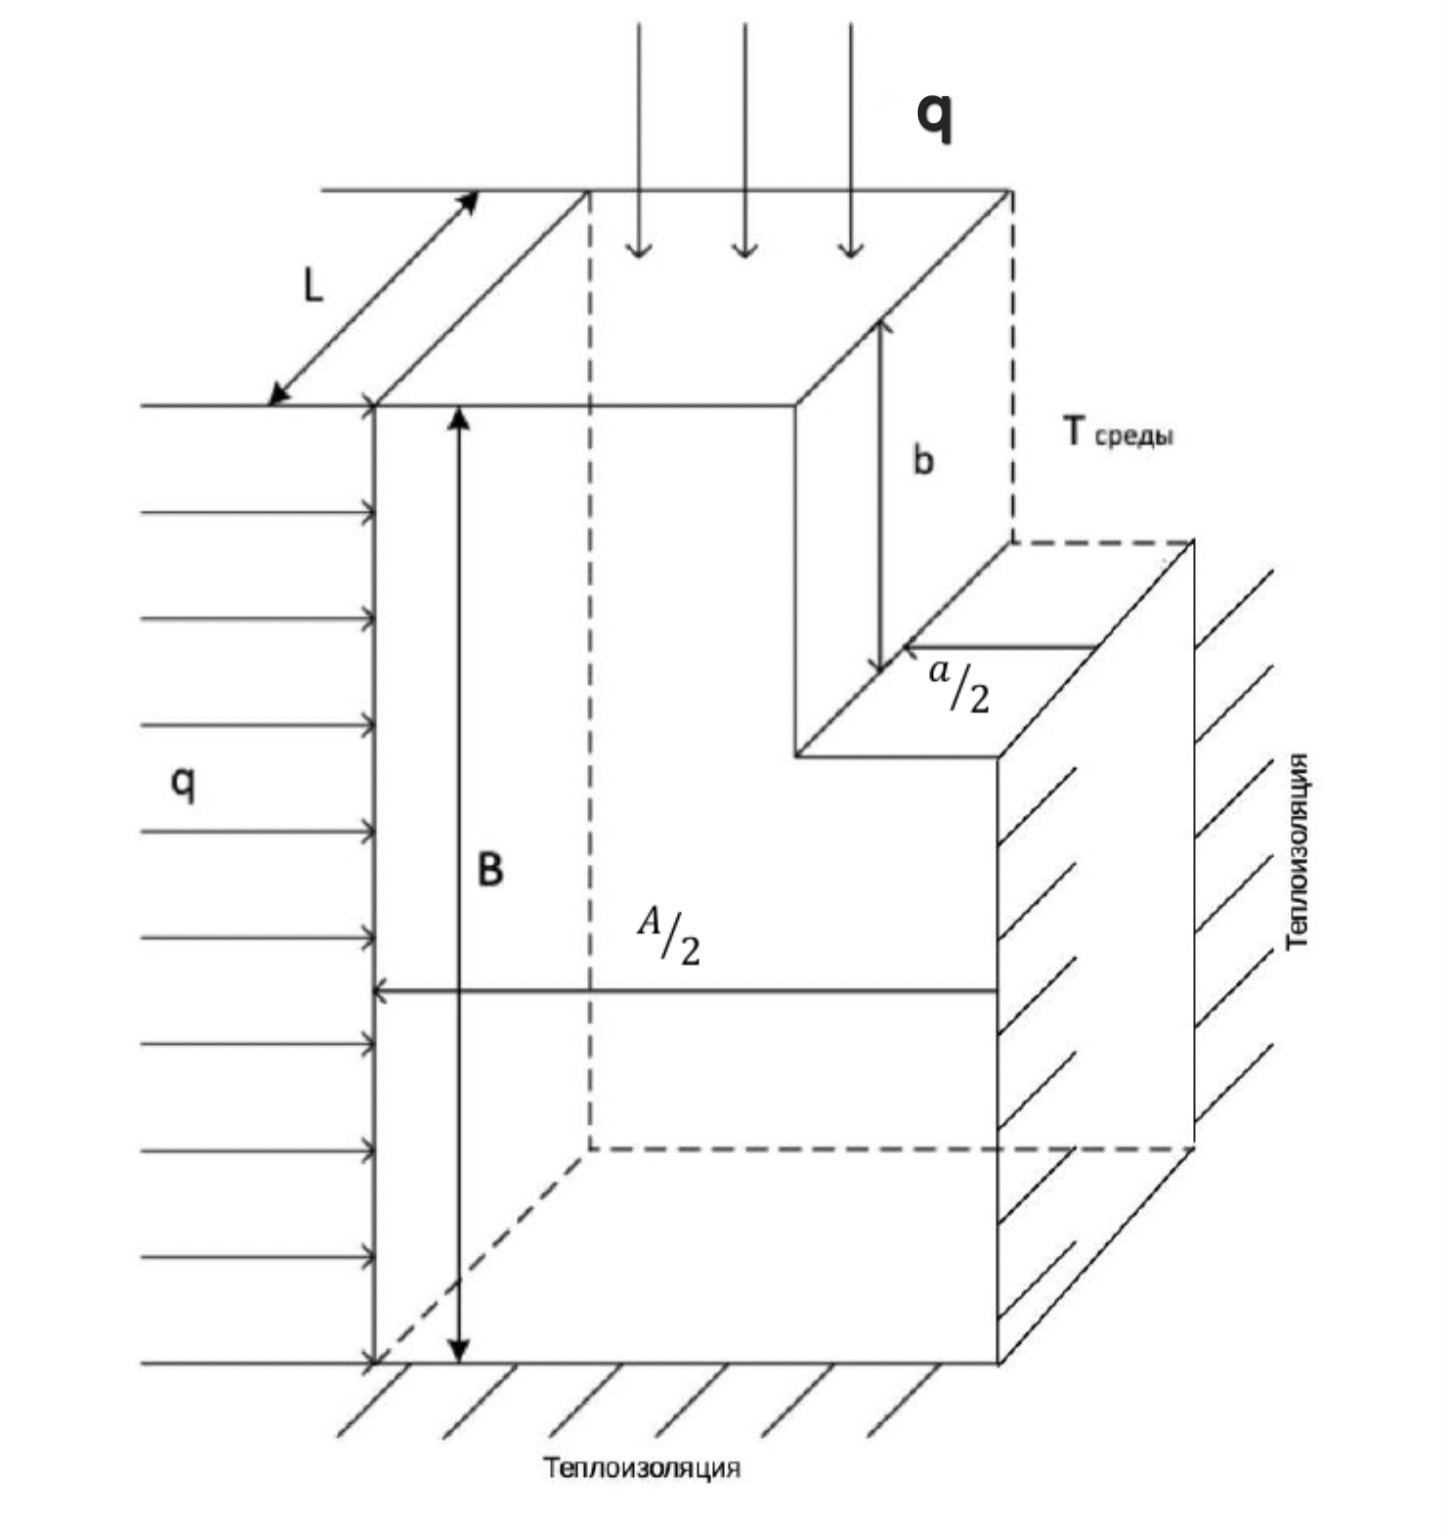
\includegraphics[width=0.5\textwidth]{img2.jpeg}
\end{center}

1. Проведем дискретизацию области дискретными одномерными элементами:

\begin{center}
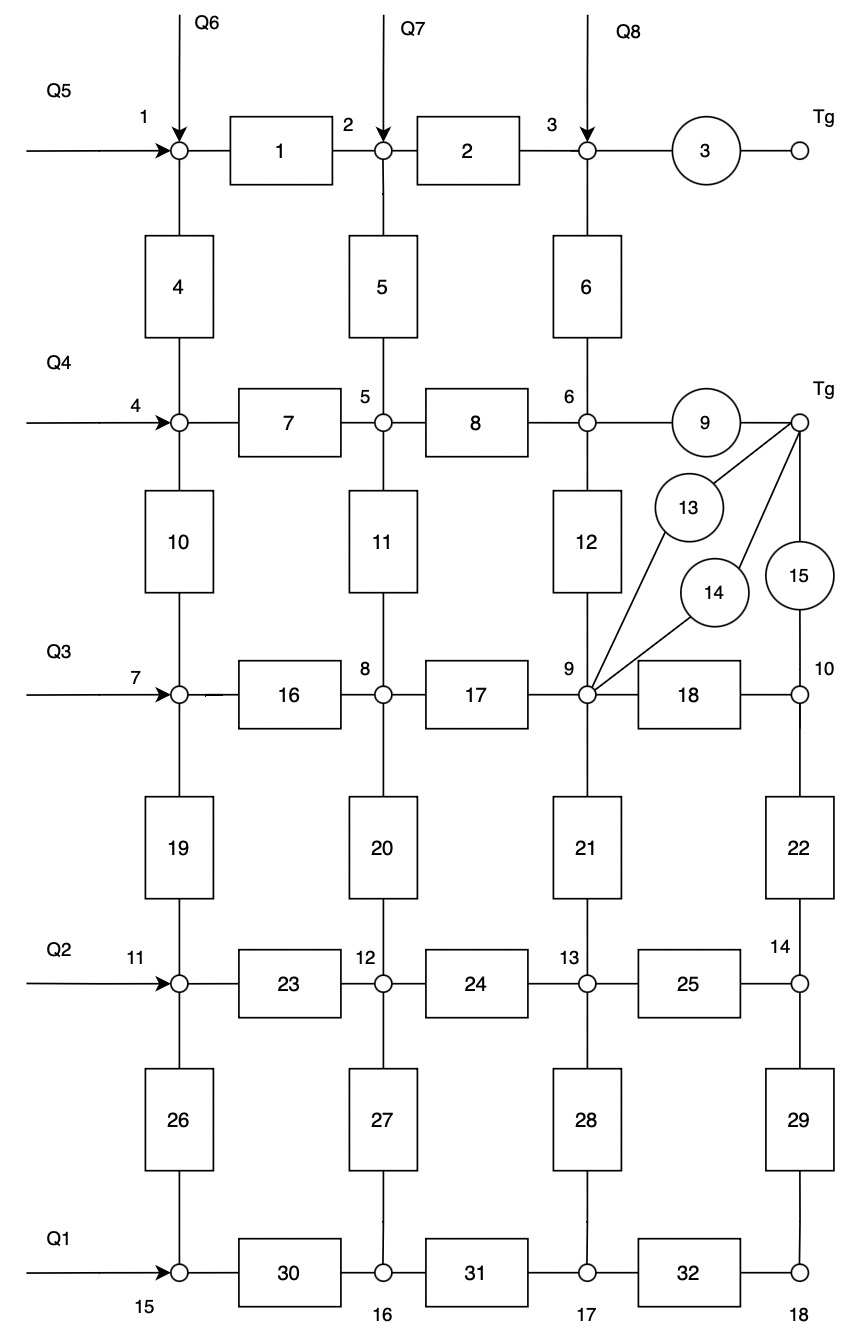
\includegraphics[width=0.5\textwidth]{img3.jpeg}
\end{center}

2-3. Выпишем уравнения равновесия для нескольких элементов. Запишем локальные матрицы для внутренних элементов, граничных элементов и локальных векторов правых частей:

Рассмотрим элемент 30: 
\begin{center}
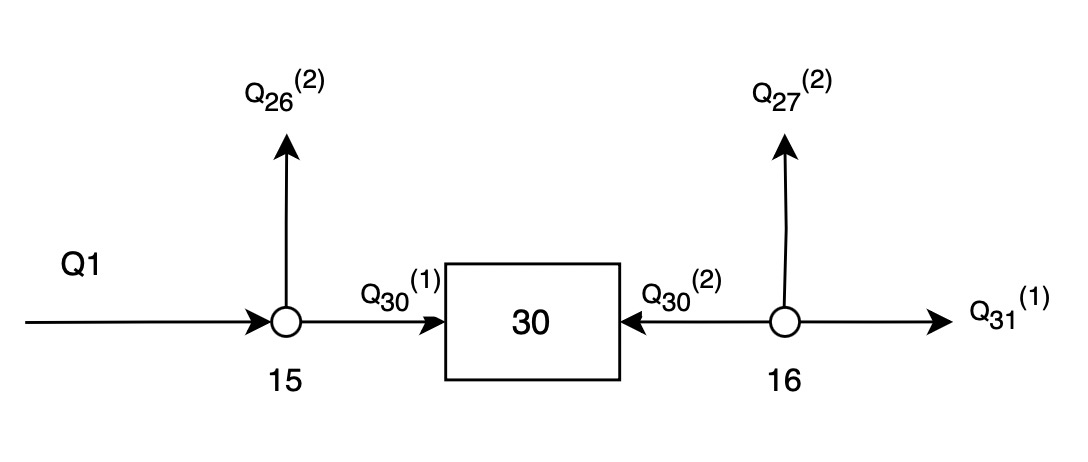
\includegraphics[width=0.5\textwidth]{img4.jpeg}
\end{center}

Составим уравнения равновесия:
\begin{equation} \label{eq1}
\begin{cases}
Q_{26}^{(2)} + Q_{30}^{(1)} = Q_1\\
Q_{30}^{(2)} + Q_{27}^{(2)} + Q_{31}^{(1)} = 0
\end{cases}
\end{equation} 

Значения потоков можно рассчитать по формулам:
\begin{equation} \label{eq2}
\begin{cases}
Q_{30}^{(1)} = k_{30} (T_{15} - T_{16})\\
Q_{30}^{(2)} =  k_{30} (T_{16} - T_{15})
\end{cases}
\end{equation} 

Подставляя \eqref{eq2} в \eqref{eq1}, получаем:
\begin{equation} \label{eq3}
\begin{cases}
k_{30} (T_{15} - T_{16}) = Q_1 - Q_{26}^{(2)}\\
 k_{30} (T_{16} - T_{15})  = -Q_{27}^{(2)} - Q_{31}^{(1)}
\end{cases}
\end{equation} 

В матричной форме:
\begin{equation} \label{eq4}
\begin{pmatrix}
k_{30} & -k_{30}\\
-k_{30} & k_{30}
\end{pmatrix}
\begin{pmatrix}
T_{15}\\
T_{16}
\end{pmatrix} =
\begin{pmatrix}
Q_1 - Q_{26}^{(2)}\\
-Q_{27}^{(2)} - Q_{31}^{(1)}
\end{pmatrix}
\end{equation} 
-- локальная матрица и локальный вектор правой части для узлов 15 и 16.

Рассмотрим элементы под номерами 2 и 3:
\begin{center}
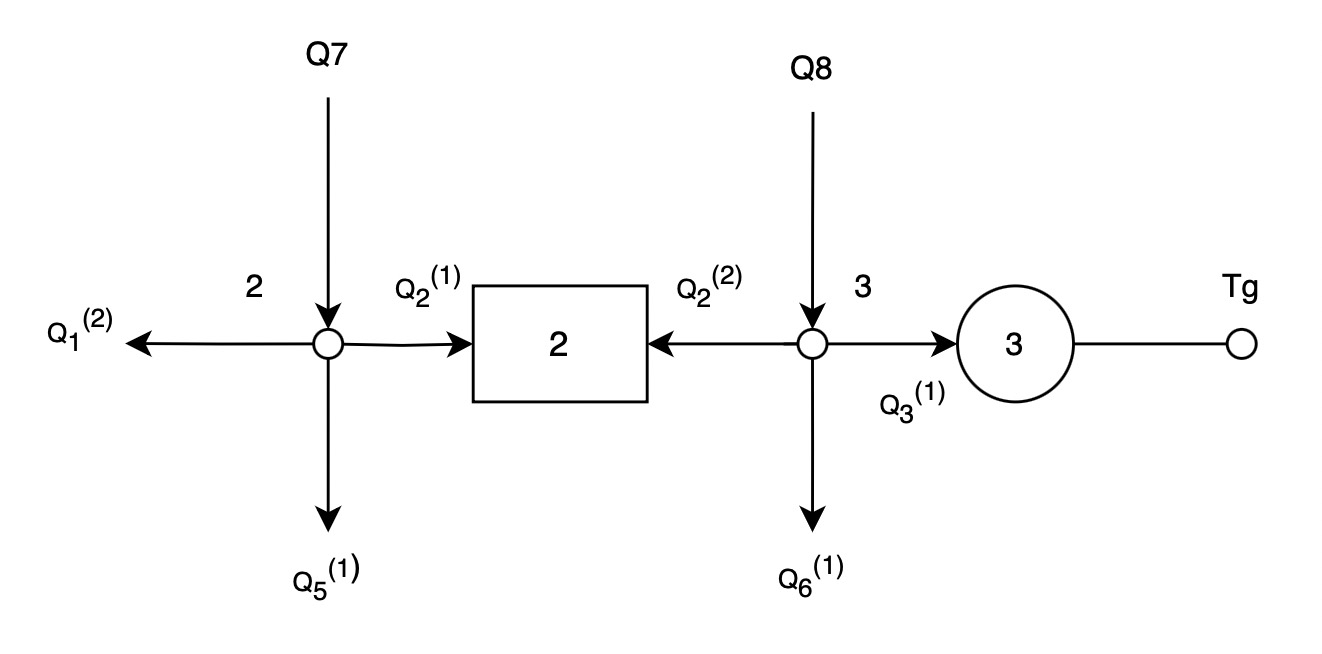
\includegraphics[width=0.5\textwidth]{img5.jpeg}
\end{center}

Составим уравнения равновесия:
\begin{equation} \label{eq5}
\begin{cases}
Q_{1}^{(2)} + Q_{2}^{(1)} + Q_{5}^{(1)} = Q_7\\
Q_{2}^{(2)} + Q_{6}^{(1)} + Q_{3}^{(1)} = Q_8
\end{cases}
\end{equation} 

Значения потоков можно рассчитать по формулам:
\begin{equation} \label{eq6}
\begin{cases}
Q_{2}^{(1)} = k_2 (T_2 - T_3)\\
Q_{2}^{(2)} = k_2 (T_3 - T_2)\\
Q_{3}^{(1)} = h_3 (T_3 - T_g)
\end{cases}
\end{equation} 

Подставляя \eqref{eq6} в \eqref{eq5}, получаем:
\begin{equation} \label{eq7}
\begin{cases}
k_2 (T_2 - T_3)  = Q_7 - Q_{1}^{(2)} - Q_{5}^{(1)}\\
k_2 (T_3 - T_2) + h_3 (T_3 - T_g) = Q_8 - Q_{6}^{(1)}
\end{cases}
\end{equation} 

В матричной форме:
\begin{equation} \label{eq8}
\begin{pmatrix}
k_{2} & -k_{2}\\
-k_{2} & k_{2} + h_3
\end{pmatrix}
\begin{pmatrix}
T_2\\
T_3
\end{pmatrix} =
\begin{pmatrix}
Q_7 - Q_{1}^{(2)} - Q_{5}^{(1)}\\
Q_8 - Q_{6}^{(1)} + h_3 T_g
\end{pmatrix}
\end{equation} 
-- локальная матрица и локальный вектор правой части для узлов 2 и 3. \\

4. Опишем процедуру формирования глобальной матрицы теплопроводности и правых частей.

Рассмотрим метод подсчета $k_i$. Согласно закону теплопроводности $k = \lambda S$, где $\lambda$ – коэффициент
теплопроводности, $S$ – площадь теплопроводящей стенки, $h$ – ее толщина. Рассматривая каждый
одномерный элемент необходимо определить его длину, а также площадь боковой поверхности, <<приходящуюся>>
на него в модели.

Остановимся на подобласти между узлами 1254. Длина элемента 1 равна 1, однако, поскольку он является граничным, на него приходится лишь половина площади подобласти:
\[k_1 = \frac{\lambda \cdot S}{h} = \lambda \cdot \frac{L \cdot b}{2\cdot2} \cdot \frac{2}{a} = \frac{\lambda}{2}\]

Для внутреннего элемента 4:
\[k_4 = \frac{\lambda \cdot S}{h} = \lambda \cdot \frac{L \cdot b}{2} \cdot \frac{2}{a} = \lambda\]

Для вычисления теплового потока, например, к узлу 2 нужно так же учитывать эту половину:
\[Q_2 = q \cdot S = \frac{q \cdot L \cdot b}{2 \cdot 2} = \frac{q}{2}\]

Составим таблицу о теплопередающей системе и глобальную матрицу теплопроводности K:
\begin{table}[h]
    \centering
    \begin{tabular}{|c|c|c|c|}
        \toprule
        Номер элемента & Характеристика элемента & Температура в & Температура во \\ 
        & & первом узле & втором узле\\ 
        \midrule
        1 & $k_1 = \lambda/2$ & $T_1$ & $T_2$\\
         \midrule
        2 & $k_2 = \lambda/2$ & $T_2$ & $T_3$\\
         \midrule
        3 & $h_3 = \alpha_g/2$ & $T_3$ & $T_g$\\
        \midrule
        4 & $k_4 = \lambda/2$ & $T_1$ & $T_4$\\
        \midrule
        5 & $k_5 = \lambda$ & $T_2$ & $T_5$\\
        \midrule
        6 & $k_6 = \lambda/2$ & $T_3$ & $T_6$\\
        \midrule
        7 & $k_7 = \lambda$ & $T_4$ & $T_5$\\
        \midrule
        8 & $k_8 = \lambda$ & $T_5$ & $T_6$\\
        \midrule
        9 & $h_9 = \alpha_g$ & $T_6$ & $T_g$\\
        \midrule
        10 & $k_{10} = \lambda/2$ & $T_4$ & $T_7$\\
        \midrule
        11 & $k_{11} = \lambda$ & $T_5$ & $T_8$\\
        \midrule
        12 & $k_{12} = \lambda/2$ & $T_6$ & $T_9$\\
        \midrule
        13 & $h_{13} = \alpha_g/2$ & $T_9$ & $T_g$\\
        \midrule
        14 & $h_{14} = \alpha_g/2$ & $T_9$ & $T_g$\\
        \midrule
        15 & $h_{15} = \alpha_g/2$ & $T_{10}$ & $T_g$\\
        \midrule
        16 & $k_{16} = \lambda$ & $T_7$ & $T_8$\\
        \midrule
        17 & $k_{17} = \lambda$ & $T_8$ & $T_9$\\
        \midrule
        18 & $k_{18} = \lambda/2$ & $T_9$ & $T_{10}$\\
        \midrule
        19 & $k_{19} = \lambda/2$ & $T_7$ & $T_{11}$\\
        \midrule
        20 & $k_{20} = \lambda$ & $T_8$ & $T_{12}$\\
        \midrule
        21 & $k_{21} = \lambda$ & $T_9$ & $T_{13}$\\
        \midrule
        22 & $k_{22} = \lambda/2$ & $T_{10}$ & $T_{14}$\\
        \midrule
        23 & $k_{23} = \lambda$ & $T_{11}$ & $T_{12}$\\
        \midrule
        24 & $k_{24} = \lambda$ & $T_{12}$ & $T_{13}$\\
        \midrule
        25 & $k_{25} = \lambda$ & $T_{13}$ & $T_{14}$\\
        \midrule
        26 & $k_{26} = \lambda/2$ & $T_{11}$ & $T_{15}$\\
        \midrule
        27 & $k_{27} = \lambda$ & $T_{12}$ & $T_{16}$\\
        \midrule
        28 & $k_{28} = \lambda$ & $T_{13}$ & $T_{17}$\\
        \midrule
        29 & $k_{29} = \lambda/2$ & $T_{14}$ & $T_{18}$\\
        \midrule
        30 & $k_{30} = \lambda/2$ & $T_{15}$ & $T_{16}$\\
        \midrule
        31 & $k_{31} = \lambda/2$ & $T_{16}$ & $T_{17}$\\
        \midrule
        32 & $k_{32} = \lambda/2$ & $T_{17}$ & $T_{18}$\\
        \bottomrule
    \end{tabular}
\end{table}

\newpage
\begin{landscape}
\begin{table}[h]
    \centering
    \begin{tabular}{|c|c|c|c|c|c|c|c|c|c|c|c|c|c|c|c|c|c|c|}
        \toprule
        &1&2&3&4&5&6&7&8&9&10&11&12&13&14&15&16&17&18\\ 
        \midrule
        1&$k_1 + k_4$&$-k_1$&0&$-k_4$&0&0&0&0&0&0&0&0&0&0&0&0&0&0\\ 
         \midrule
        2& $-k_1$ & $k_1 + k_2 +$ &$-k_2$&0&$-k_5$&0&0&0&0&0&0&0&0&0&0&0&0&0\\ 
        && $+ k_5$ &&&&&&&&&&&&&&&\\
         \midrule
        3&0&$-k_2$& $k_2 + k_6 + $ &0&0&$-k_6$&0&0&0&0&0&0&0&0&0&0&0&0\\ 
      &&& $+ h_3$ &&&&&&&&&&&&&&\\
        \midrule
        4&$-k_4$&0&0& $k_4 + k_7 + $ &$-k_7$&0&$-k_{10}$&0&0&0&0&0&0&0&0&0&0&0\\ 
        &&&& $+ k_{10}$ &&&&&&&&&&&&&\\
        \midrule
        5&0&$-k_5$&0&$-k_7$& $k_5 + k_7 +$ &$-k_8$&0&$-k_{11}$&0&0&0&0&0&0&0&0&0&0\\ 
        &&&&& $+ k_8 + k_{11} $&&&&&&&&&&&&\\
        \midrule
        6&0&0&$-k_6$&0&$-k_8$& $k_6 + k_8 + $ &0&0&$-k_{12}$&0&0&0&0&0&0&0&0&0\\ 
        &&&&&& $+ k_{12} + h_9 $&&&&&&&&&&&\\
        \midrule
        7&0&0&0&$-k_{10}$&0&0& $k_{10} + k_{16} + $ &$-k_{16}$&0&0&$-k_{19}$&0&0&0&0&0&0&0\\ 
        &&&&&&& $+ k_{19} $&&&&&&&&&&\\
        \midrule
        8&0&0&0&0&$-k_{11}$&0&$-k_{16}$& $k_{11} + k_{16} + $ &$-k_{17}$&0&0&$-k_{20}$&0&0&0&0&0&0\\ 
        &&&&&&&& $+ k_{17} + k_{20} $&&&&&&&&&\\
        \midrule
        9&0&0&0&0&0&$-k_{12}$&0&$-k_{17}$& $k_{12} + k_{17} + k_{18} + $ &$-k_{18}$&0&0&$-k_{21}$&0&0&0&0&0\\ 
        &&&&&&&&& $+ k_{21} + h_{13} + h_{14} $&&&&&&&&\\
        \midrule
        10&0&0&0&0&0&0&0&0&$-k_{18}$& $k_{18} + k_{22} + $ &0&0&0&$-k_{22}$&0&0&0&0\\ 
        &&&&&&&&&& $+ h_{15} $&&&&&&&\\
        \midrule
        11&0&0&0&0&0&0&$-k_{19}$&0&0&0& $k_{19} + k_{23} + $ &$-k_{23}$&0&0&$-k_{26}$&0&0&0\\ 
        &&&&&&&&&&& $+ k_{26} $&&&&&&\\
        \midrule
        12&0&0&0&0&0&0&0&$-k_{20}$&0&0&$-k_{23}$& $k_{20} + k_{23} + $ &$-k_{24}$&0&0&$-k_{27}$&0&0\\ 
        &&&&&&&&&&&& $+ k_{24} + k_{27} $&&&&&\\
                \midrule
        13&0&0&0&0&0&0&0&0&$-k_{21}$&0&0&$-k_{24}$& $k_{21} + k_{24} + $ &$-k_{25}$&0&0&$-k_{28}$&0\\ 
        &&&&&&&&&&&&& $+ k_{25} + k_{28}$&&&&\\
        \midrule
        14 & 0&0&0&0&0&0&0&0&0&$-k_{22}$&0&0&$-k_{25}$& $k_{22} + k_{25} + $ &0&0&0&$k_{29}$\\ 
        &&&&&&&&&&&&&& $+ k_{29}$&&&\\
        \midrule
        15 & 0&0&0&0&0&0&0&0&0&0&$-k_{26}$&0&0&0& $k_{26} + k_{30} $ &0&0&0\\ 
        \midrule
        16 & 0&0&0&0&0&0&0&0&0&0&0&$-k_{27}$&0&0&0& $k_{27} + k_{30} + $ &$-k_{31}$&0\\ 
        &&&&&&&&&&&&&&&& $+ k_{31}$&\\
        \midrule
        17 & 0&0&0&0&0&0&0&0&0&0&0&0&$-k_{28}$&0&0&$-k_{31}$& $k_{28} + k_{31} $ &$-k_{32}$\\ 
        &&&&&&&&&&&&&&&&& $+ k_{32}$\\
        \midrule
        18 & 0&0&0&0&0&0&0&0&0&0&0&0&0&$-k_{29}$&0&0&$-k_{32}$& $k_{29} + k_{32}$\\ 
               \bottomrule
    \end{tabular}
\end{table}

\end{landscape}

\newpage
Правые части:
\begin{table}[h]
    \centering
    \begin{tabular}{|c|c|c|c|c|c|c|c|c|c|c|c|c|c|}
        \toprule
        1&2&3&4&5&6&7&8&9&10&11&12&13\\ 
        \midrule
        $Q_5 + Q_6$& $Q_7$ & $Q_8 + h_3 T_g$ & $Q_4$& 0 & $h_9 T_g$ & $Q_3$ &0 & $h_{13} T_g + h_{14} T_g$ & $h_{15} T_g$ & $Q_2$ & 0 &0\\ 
  \bottomrule
    \end{tabular}
\end{table}
\begin{table}[h]
    \centering
    \begin{tabular}{|c|c|c|c|c|}
        \toprule
        14&15&16&17&18\\ 
        \midrule
        0 & $Q_1$ &0 &0 &0\\ 
  \bottomrule
    \end{tabular}
\end{table}

\[Q_1 = \frac{q}{2},\ Q_2 = q,\ Q_3 = q,\ Q_4 = q,\ Q_5 = \frac{q}{2},\ Q_6 = \frac{q}{2},\ Q_7 = q,\ Q_8 = \frac{q}{2}\]
\[Q = \left[\begin{matrix}150.0\\150.0\\275.0\\150.0\\0.0\\125.0\\150.0\\0.0\\250.0\\125.0\\150.0\\0.0\\0.0\\0.0\\75.0\\0.0\\0.0\\0.0\end{matrix}\right]\]

\begin{landscape}
\[
K = 
\left[\begin{array}{cccccccccccccccccc}75.0 & -37.5 & 0.0 & -37.5 & 0.0 & 0.0 & 0.0 & 0.0 & 0.0 & 0.0 & 0.0 & 0.0 & 0.0 & 0.0 & 0.0 & 0.0 & 0.0 & 0.0\\-37.5 & 150.0 & -37.5 & 0.0 & -75.0 & 0.0 & 0.0 & 0.0 & 0.0 & 0.0 & 0.0 & 0.0 & 0.0 & 0.0 & 0.0 & 0.0 & 0.0 & 0.0\\0.0 & -37.5 & 80.0 & 0.0 & 0.0 & -37.5 & 0.0 & 0.0 & 0.0 & 0.0 & 0.0 & 0.0 & 0.0 & 0.0 & 0.0 & 0.0 & 0.0 & 0.0\\-37.5 & 0.0 & 0.0 & 150.0 & -75.0 & 0.0 & -37.5 & 0.0 & 0.0 & 0.0 & 0.0 & 0.0 & 0.0 & 0.0 & 0.0 & 0.0 & 0.0 & 0.0\\0.0 & -75.0 & 0.0 & -75.0 & 300.0 & -75.0 & 0.0 & -75.0 & 0.0 & 0.0 & 0.0 & 0.0 & 0.0 & 0.0 & 0.0 & 0.0 & 0.0 & 0.0\\0.0 & 0.0 & -37.5 & 0.0 & -75.0 & 160.0 & 0.0 & 0.0 & -37.5 & 0.0 & 0.0 & 0.0 & 0.0 & 0.0 & 0.0 & 0.0 & 0.0 & 0.0\\0.0 & 0.0 & 0.0 & -37.5 & 0.0 & 0.0 & 150.0 & -75.0 & 0.0 & 0.0 & -37.5 & 0.0 & 0.0 & 0.0 & 0.0 & 0.0 & 0.0 & 0.0\\0.0 & 0.0 & 0.0 & 0.0 & -75.0 & 0.0 & -75.0 & 300.0 & -75.0 & 0.0 & 0.0 & -75.0 & 0.0 & 0.0 & 0.0 & 0.0 & 0.0 & 0.0\\0.0 & 0.0 & 0.0 & 0.0 & 0.0 & -37.5 & 0.0 & -75.0 & 235.0 & -37.5 & 0.0 & 0.0 & -37.5 & 0.0 & 0.0 & 0.0 & 0.0 & 0.0\\0.0 & 0.0 & 0.0 & 0.0 & 0.0 & 0.0 & 0.0 & 0.0 & -37.5 & 80.0 & 0.0 & 0.0 & 0.0 & -37.5 & 0.0 & 0.0 & 0.0 & 0.0\\0.0 & 0.0 & 0.0 & 0.0 & 0.0 & 0.0 & -37.5 & 0.0 & 0.0 & 0.0 & 150.0 & -75.0 & 0.0 & 0.0 & -37.5 & 0.0 & 0.0 & 0.0\\0.0 & 0.0 & 0.0 & 0.0 & 0.0 & 0.0 & 0.0 & -75.0 & 0.0 & 0.0 & -75.0 & 300.0 & -75.0 & 0.0 & 0.0 & -75.0 & 0.0 & 0.0\\0.0 & 0.0 & 0.0 & 0.0 & 0.0 & 0.0 & 0.0 & 0.0 & -37.5 & 0.0 & 0.0 & -75.0 & 300.0 & -75.0 & 0.0 & 0.0 & -75.0 & 0.0\\0.0 & 0.0 & 0.0 & 0.0 & 0.0 & 0.0 & 0.0 & 0.0 & 0.0 & -37.5 & 0.0 & 0.0 & -75.0 & 150.0 & 0.0 & 0.0 & 0.0 & -37.5\\0.0 & 0.0 & 0.0 & 0.0 & 0.0 & 0.0 & 0.0 & 0.0 & 0.0 & 0.0 & -37.5 & 0.0 & 0.0 & 0.0 & 75.0 & -37.5 & 0.0 & 0.0\\0.0 & 0.0 & 0.0 & 0.0 & 0.0 & 0.0 & 0.0 & 0.0 & 0.0 & 0.0 & 0.0 & -75.0 & 0.0 & 0.0 & -37.5 & 150.0 & -37.5 & 0.0\\0.0 & 0.0 & 0.0 & 0.0 & 0.0 & 0.0 & 0.0 & 0.0 & 0.0 & 0.0 & 0.0 & 0.0 & -75.0 & 0.0 & 0.0 & -37.5 & 150.0 & -37.5\\0.0 & 0.0 & 0.0 & 0.0 & 0.0 & 0.0 & 0.0 & 0.0 & 0.0 & 0.0 & 0.0 & 0.0 & 0.0 & -37.5 & 0.0 & 0.0 & -37.5 & 75.0\end{array}\right]
\]

\end{landscape}

\newpage

4-5. СЛАУ и ее решение \\

СЛАУ соответствующая постановке задачи имеет вид:
\[K \overline t = \overline f,\]
где $\overline t$ – вектор температур в узлах области. \\

Данную СЛАУ можно решить с помощью разложения
Холецкого с последующим применением метода Гаусса. 
Разложение Холецкого позволяет представить матрицу $K = (k_{ij})$ в виде $K=LL^T$ , где $L = (l_{ij})$ – нижнетреугольная матрица. Разложение Холецкого имеет следующие рабочие формулы:
\[
\begin{cases}
l_{11} = \sqrt{k_{11}},\\
l_{j1} = \frac{k_{j1}}{l_{11}},\ j = 2, \dots, n,\\
l_{ii} = \sqrt{k_{ii} - \sum \limits_{p=1}^{i-1} l_{ip}^2}, \ i = 2, \dots, n,\\
l_{ji} = \frac{1}{l_{ii}} \left( k_{ji} - \sum \limits_{p=1}^{i-1} l_{ip} l_{jp} \right),\ i = 2, \dots, n-1,\ j = i+1, \dots, n\\
\end{cases}
\]

Если же имеется СЛАУ вида $K \overline t = \overline f$, то решение данной СЛАУ, применив разложение
Холецкого $K=LL^T$, можно получить следующие СЛАУ:
\[L \overline y = \overline f,\ L^T \overline t = \overline y.\]

Поскольку матрицы $L$ и $L^T$ являются нижне- и верхнетреугольной соответственно, для решения
СЛАУ применим метод Гаусса.

Решая СЛАУ данным методом, получим следующее распределение температур в узлах системы дискретных одномерных элементов:

\begin{table}[h]
    \centering
    \begin{tabular}{|c|c|c|c|c|c|c|c|c|c|}
        \toprule
        $T_1$&$T_2$&$T_3$&$T_4$&$T_5$&$T_6$&$T_7$&$T_8$&$T_9$&$T_{10}$\\ 
        \midrule
        35.07& 33.44& 30.01& 32.7 & 32.34& 23.26& 27.06& 23.78& 14.93& 15.85 \\ 
  \bottomrule	
    \end{tabular}
\end{table}
\begin{table}[h]
    \centering
    \begin{tabular}{|c|c|c|c|c|c|c|c|}
        \toprule
        $T_{11}$&$T_{12}$&$T_{13}$&$T_{14}$&$T_{15}$&$T_{16}$&$T_{17}$&$T_{18}$\\ 
        \midrule
        23.96& 20.81& 15.13& 15.56& 23.16& 20.37& 16.69& 16.12 \\ 
  \bottomrule
    \end{tabular}
\end{table}

\begin{center}
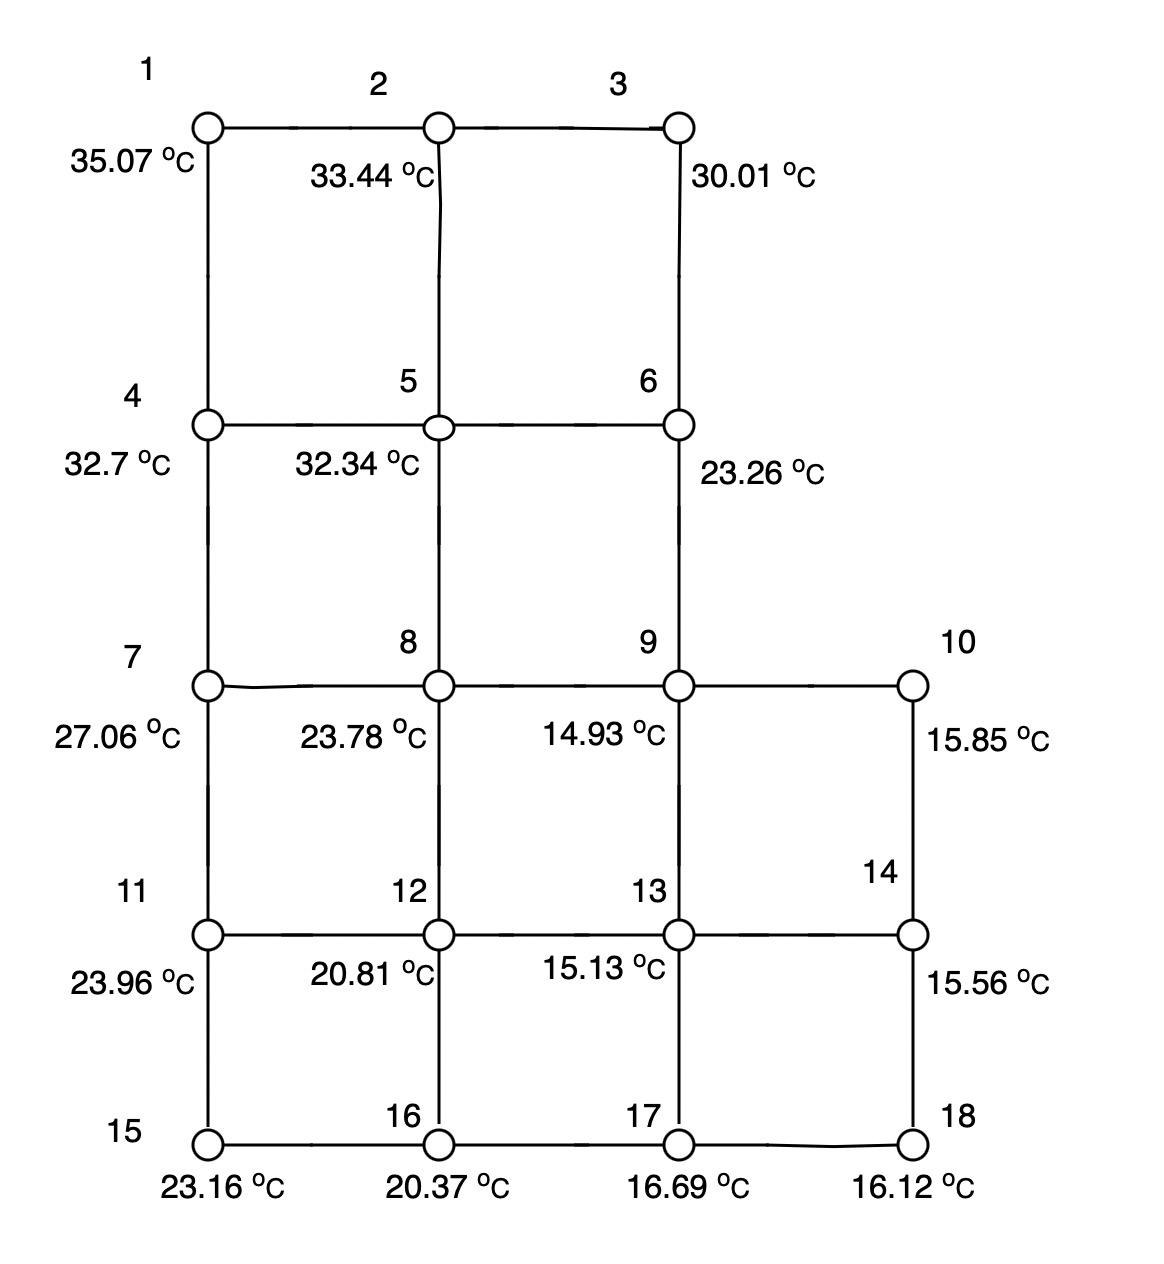
\includegraphics[width=0.5\textwidth]{imgT.jpeg}
\end{center}






































\end{document}